\section{Nonadiabatic friction / Electron-phonon calculations}\label{Sec:Friction}

\emph{THIS MODULE IS CURRENTLY UNDER DEVELOPMENT AND FUNCTIONALITY AND KEYWORDS WILL CHANGE FREQUENTLY OVER THE NEXT VERSIONS.}\\
For questions please directly contact reinhard.maurer@yale.edu.

This module calculates the electronic friction tensor due to the nonadiabatic or electron-phonon coupling. This yields vibrational lifetimes and classical friction forces that can be used in molecular dynamics with nonadiabatic friction in a Langevin formalism, but also as input to calculate electron-phonon coupling constants.

The key references you should consult are:

\begin{itemize}
 \item Ab-initio tensorial electronic friction for molecules on metal surfaces: nonadiabatic vibrational relaxation
 R. J. Maurer, M. Askerka, V. S. Batista, J. C. Tully, arXiv:1607.02650 (2016)
 \item Role of Tensorial Electronic Friction in Energy Transfer at Metal surfaces
 M. Askerka, R. J. Maurer, V. S. Batista, J. C. Tully, Phys. Rev. Lett. 116, 217601 (2016)
\end{itemize}

\subsection*{Theory}

Typically, for molecular dynamics at ambient conditions, the Born-Oppenheimer approximation is well justified. This means that the time scales of electronic and nuclear motion are well separated. This is the case for most thermal reactions of molecules in gas phase or for insulating or semi-conducting materials. Therefore nuclei can be viewed as moving on a single potential energy surface (PES) given by the ground state electronic structure. This is, however, not the case for nuclei moving on or in metal surfaces (see Fig.~\ref{fig:friction}). The continuum of electronic states in metals can already be excited by the vibrational motion of the adsorbate atoms due to resonance at similar energy scales. As a result adsorbate atoms exhibit additional frictional forces. Another way to view this is that the vibrations or phonons are being screened by electronic excitations giving them a finite lifetime. Assuming that the ground and excited state PES are parallel and that these adiabatic effects are only weakly perturbing the adsorbate nuclear motion, we can apply perturbation theory to this problem. 

\begin{figure}
 \centering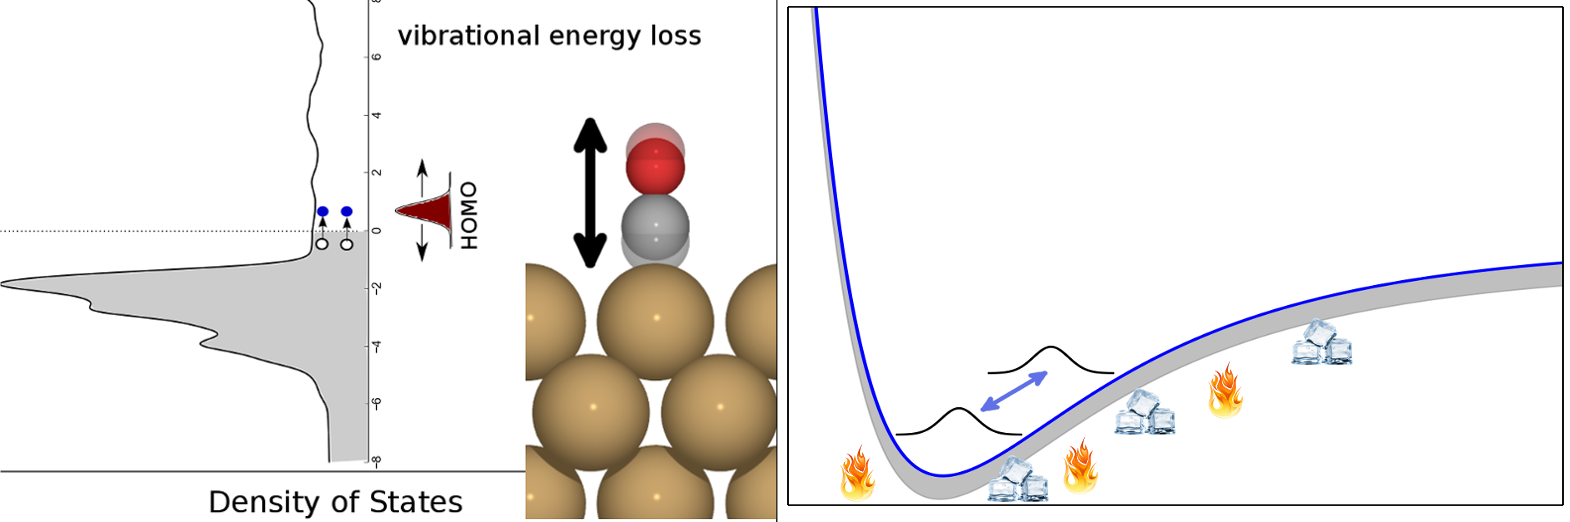
\includegraphics{friction.png}
 \caption{\label{fig:friction} left: Schematic view of adsorbate vibration (here shown for a CO molecule on a Cu(100) surface) leading to changes in the electronic structure that excite electron-hole pairs from below to above the Fermi level of the metal density-of-states. right: In the Langevin picture of electronic friction, these electron-hole pairs act as energy gain or loss channels on the nuclear motion along a single potential energy surface.}
\end{figure}

The picture in Fig.~\ref{fig:friction} holds if:
\begin{itemize}
 \item the coupling is weak compared to the individual contributions of electrons and nuclei, and if
 \item electron-hole pair excitations do not lead to a qualitative change in the nuclear dynamics.
\end{itemize}

Following first order time-dependent perturbation theory or many-body perturbation theory (using  lowest order RPA) one arrives at the Fermi's golden rule expression for relaxation rate along a vibration with frequency $\omega_j$:
\begin{align}\label{eq-Gamma}
 \Gamma(\omega_{j}) =\frac{\pi\hbar^2\omega_{j}}{M}\sum_{\mathbf{k},\nu,\nu'>\nu} 
    |g_{\mathbf{k}\nu,\nu'}^{j}|^2 \cdot
   [f(\epsilon_{\mathbf{k}\nu})-f(\epsilon_{\mathbf{k}\nu'})]\cdot \delta(\epsilon_{\mathbf{k}\nu'}-\epsilon_{\mathbf{k}\nu}-\hbar\omega_{j}),
\end{align}
with 
\begin{align}\label{eq-g}
g_{\mathbf{k}\nu,\nu'}^{j} = \braket{\psi_{\mathbf{k}\nu}|\mathbf{e}_{j}\cdot\mathbf{\nabla}_{\mathbf{R}}|\psi_{\mathbf{k}\nu'}}.
\end{align}
The relaxation rate $\Gamma$ defines the lifetime of the mode $\tau=1/\Gamma$ and the vibrational linewidth $\gamma = \Gamma\hbar$. In eq.~\ref{eq-g}, $\mathbf{e}_{j}$ is the atomic displacement vector corresponding to the vibrational normal mode $\omega_{j}$ and $\mathbf{\nabla}_{\mathbf{R}}$ is the vector of Cartesian derivatives. 

This can be rewritten in terms of cartesian displacements.
\begin{align}\label{eq-Gamma3}
  \Gamma(\omega_{j}) &= \frac{1}{M} \mathbf{e}^T_{j}\cdot \biggl( \pi\hbar\sum_{\mathbf{k},\nu,\nu'>\nu} \braket{\psi_{\mathbf{k}\nu}|\frac{\partial}{\partial R_{n'a'}}|\psi_{\mathbf{k}\nu'}}\braket{\psi_{\mathbf{k}\nu'}|\frac{\partial}{\partial R_{na}}|\psi_{\mathbf{k}\nu}}\cdot (\epsilon_{\mathbf{k}\nu'}-\epsilon_{\mathbf{k}\nu}) \cdot  \\ \nonumber &    [f(\epsilon_{\mathbf{k}\nu})-f(\epsilon_{\mathbf{k}\nu'})]\cdot\delta(\epsilon_{\mathbf{k}\nu'}-\epsilon_{\mathbf{k}\nu}-\hbar\omega_j) \biggr) \cdot \mathbf{e}_{j}
\end{align}

Correspondingly the rate of decay of adsorbate motion along a displacement vector $\mathbf{e}_{\mathbf{j}}$ is given by:
\begin{equation}
  \Gamma(\omega_{j}) =\mathbf{e}^T_{j}\cdot\tilde{\mathbf{\Lambda}}(\omega_j)\cdot\mathbf{e}_{j}. 
\end{equation}
where $\tilde{\Lambda}$ is the so-called mass-weighted friction tensor or tensor of nonadiabatic relaxation rates $\tilde{\Lambda}_{ij}=\Lambda_{ij}/(\sqrt{m_i}\sqrt{m_j})$. 

In practice the friction tensor is calculated using the ground state Kohn-Sham eigenstates and evaluated in the quasi-static or zero-frequency limit as $\Lambda(\omega\rightarrow0)$. This can be done for a cluster and a periodic system. In the periodic case, the relaxation rate of periodic motion ($q=0$, default) can be calculated or, in combination with DFPT, averaged over the whole phonon Brillouin zone ($\int_{\mathbf{q}} \mathbf{\Lambda}(\mathbf{q})\delta(\omega-\omega_{\mathbf{q}})$ (work in progress). The matrix elements are expressed in the local atomic orbital basis by derivatives with respect to the Hamiltonian and overlap matrix in basis representation (see references for more details).

The implementation in FHI-Aims collects all excitations from occupied to unoccupied states in a window of \keyword{friction\_max\_energy} close to the Fermi level into a discretized electron-phonon spectral function (with discretization length \keyword{friction\_discretization\_length}) and applies a Gaussian broadening of \keyword{friction\_broadening\_width} to facilitate convergence with respect to $\mathbf{k}$-points. The corresponding spectral functions along every pair of cartesian components can be printed in file 'nacs-spectrum.out', but as default only the final friction tensor evaluated at zero frequency is printed in 'friction\_tensor.out'. Calculations need to be converged with respect to the number of k points. Convergence is achieved if the relaxation rate is stable over a large range of \keyword{friction\_broadening\_width} values (10\% variation over 0.3-0.6 eV).

In order to do this, first the coupling matrix elements need to be calculated. This can be done using finite difference displacements of the involved atoms or Density Functional Perturbation Theory (see \keyword{calculate\_friction}). 

%%%Langevin Dynamics

% Head-Gordon and Tully were able to show that, starting from the Ehrenfest approximation, using classical auxiliary coordiantes for the electrons, one can derive nuclear motion, which exhibits frictional forces due to the non-adiabatic coupling with the electronic structure. The corresponding equations of motion are:
%eq
% Here the friction tensor defines the friction forces and due to the fluctuation-dissipation theorem random statistical white noise force appear as $S$.


% \subsection*{Working equations and approximations}

% TODO

\subsection*{Calculation workflow and functionality}

The electron-phonon calculation in FHI-aims involves following steps:
\begin{enumerate}
 \item SCF calculation.
 \item Finite-difference or DFPT (in progress) calculation of matrix elements. Optionally, these matrix elements can be read from files.
 \item Calculate relaxation rates and line widths from electronic structure data.
\end{enumerate}

The module currently allows to:
\begin{itemize}
 \item calculate the nonadiabatic relaxation rate tensor in the quasi-static limit using finite-difference matrix elements for cluster and PBC systems. The latter only works for the Gamma point ($q=0$).
 \item atomwise input and output nonadiabatic coupling matrix elements, which can serve as a restart mechanism
 \item DFPT evaluation of overlap derivatives for the cluster case. Coupling to the DFPT module an extension to phonon wavevectors beyond the $q=0$ point is work in progress.
\end{itemize}

\subsection*{Tags for general section of \texttt{control.in}}

\keydefinition{calculate\_friction}{control.in} {
\noindent
Usage: \keyword{calculate\_friction} \option{type}\\
Purpose: Triggers the calculation of the friction tensor.\\
\option{type}: String that defines the type of calculation to be performed.
\begin{itemize}
\item numerical\_friction: Using finite difference to calculate matrix elements. default
\item DFPT: Using Density Functional Perturbation Theory to calculate matrix elements (currently only for pz-lda and n\_spin=1, see DFPT chapter)
\end{itemize}
}

With the keyword \option{type} the user can specify the calculation mode for the evaluation of electron-phonon coupling matrix elements.\\
In addition, the keyword \keyword{empty\_states} should be set to a large number, or the keyword \keyword {calculate\_all\_eigenstates} should be used, to make sure the code generates all possible empty states provided from the basis set. This number will also be reduced automatically by the code to the maximum number that can be generated from the basis set.


% \keydefinition{friction\_delta\_type}{control.in} {
% \noindent
% Usage: \keyword{friction\_delta\_type} \option{type}\\
% Purpose: Specify the broadening scheme used to calculate the density of states.\\
% \option{type}: String that defines the broadening scheme
% \begin{itemize}
% \item square: Uses a square window
% \item gaussian: Uses a Gaussian window [default]
% \item lorentzian: Uses a Lorentzian window
% \item sine: Uses a sine$^2$/x$^2$ function
% \item squashed\_fermi: Uses a  
% \item methfessel: Uses the Methfessel-Paxton scheme  \\
% 
% \end{itemize}
% }

\keydefinition{friction\_numeric\_disp}{control.in} {
\noindent
Usage: \keyword{friction\_numeric\_disp} \option{disp}\\
Purpose: This keyword provides the finite difference displacement stencil \option{disp} in \AA{} for numerical calculation of the friction tensor. The default is 0.0025~\AA.
}

\keydefinition{friction\_broadening\_width}{control.in} {
\noindent
Usage: \keyword{friction\_broadening\_width} \option{width}\\
Purpose: This keyword specifies the width of the broadening function that is used to average over the spectral function and to facilitate Brillouin zone integration. The typical range is 0.3 to 0.6~eV. The default value is 0.3 eV.\\
}

\keydefinition{friction\_temperature}{control.in} {
\noindent
Usage: \keyword{friction\_temperature} \option{float}\\
Purpose: This keyword specifies the electronic temperature in Kelvin that enters through state occupations in Fermi's rolden rule. The default value is 300~K.  \\
}

\keydefinition{friction\_iter\_limit}{control.in} {
\noindent
Usage: \keyword{friction\_iter\_limit} \option{integer}\\
Purpose: This keyword specifies the maximum number of iterations in the finite-difference or DFPT evaluation of electron-phonon matrix elements. The default value is 20. \\
}

\keydefinition{friction\_accuracy\_rho}{control.in} {
\noindent
Usage: \keyword{friction\_accuracy\_rho} \option{float}\\
Purpose: This keyword specifies the accuracy to which the electronic density is converged in the finite difference calculation. The default is 0.00001.\\
}

\keydefinition{friction\_accuracy\_etot}{control.in} {
\noindent
Usage: \keyword{friction\_accuracy\_etot} \option{float}\\
Purpose: This keyword specifies the accuracy to which the electronic energy is converged in the finite difference calculation. The default is 0.00001~eV.\\
}

\keydefinition{friction\_accuracy\_eev}{control.in} {
\noindent
Usage: \keyword{friction\_accuracy\_eev} \option{float}\\
Purpose: This keyword specifies the accuracy to which the sum of Kohn-Sham eigen energies is converged in the finite difference calculation. The default is 0.01~eV.\\
}

\keydefinition{friction\_accuracy\_potjump}{control.in} {
\noindent
Usage: \keyword{friction\_accuracy\_potjump} \option{float}\\
Purpose: This keyword specifies the accuracy to which the potential is converged in the finite difference calculation. The default is 1.01~eV.\\
}

\keydefinition{friction\_delta\_type}{control.in} {
\noindent
Usage: \keyword{friction\_delta\_type} \option{type}\\
Purpose: This keyword specifies the shape of the broadening function that is used to generate a converged electron-phonon spectral function. The default type is a gaussan function. Choices include a gaussian function (\option{gaussian}, a square window (\option{square}), a squashed Fermi function (\option{squashed\_fermi}), a Lorentzian (\option{lorentzian}), and a sine function (\option{sine}).\\
}

\keydefinition{friction\_max\_energy}{control.in} {
\noindent
Usage: \keyword{friction\_max\_energy} \option{energy}\\
Purpose: This keyword sets the maximum excitation energy in eV for which electronic excitations will be included. The safe default is 5 times the value of \keyword{friction\_broadening\_width}. It should not be below 1~eV. \\
}

\keydefinition{friction\_coupling\_matrix\_mode}{control.in} {
\noindent
Usage: \keyword{friction\_coupling\_matrix\_mode} \option{integer}\\
Purpose: This keyword sets the expression with which the coupling matrix elements are constructed from first order overlap and first order hamiltonian. There are three different modes (0 = "Head-Gordon-Tully-type", 1="Averaged-type", 2="exact matrix elements"). The default is 0. Type 2 only works in combination with DFPT. For details on the different types, please refer to the above publication reference. \\
}

\subsubsection{Output of spectral function}

\keydefinition{friction\_output\_spectrum}{control.in} {
\noindent
Usage: \keyword{friction\_output\_spectrum} \option{boolean}\\
Purpose: This keyword controls the output of the electron-phonon response as a function of energy. \\ 
\option{boolean}: .true. or .false.\\
}

\keydefinition{friction\_window\_size}{control.in} {
\noindent
Usage: \keyword{friction\_window\_size} \option{width}\\
Purpose: This keyword sets the evaluation window when calculating the full vibronic spectral function with \keyword{friction\_output\_spectrum}. There is typically no need to change this value. The default value is 0.01~\AA. \\
}

\keydefinition{friction\_discretization\_length}{control.in} {
\noindent
Usage: \keyword{friction\_window\_size} \option{width}\\
Purpose: This keyword sets the discretization of the grid on which the electron-phonon response will be printed with keyword \keyword{friction\_output\_spectrum}. The default value is 0.01~\AA. \\
}


% \keydefinition{friction\_knotk}{control.in} {
% \noindent
% Usage: \keyword{friction\_knotk} \option{boolean}\\
% Purpose: TODO\\
% \option{boolean}: .true. or .false.\\
% }

\subsubsection{Input and Output of matrix elements and vectors}

\keydefinition{friction\_read\_matrices}{control.in} {
\noindent
Usage: \keyword{friction\_read\_matrices} \option{boolean}\\
Purpose: This keyword leads to skipping the evaluation of electron-phonon matrix elements. FHI-aims will read the matrix elements from files, generated by the keyword \keyword{output friction\_matrices}.\\
\option{boolean}: .true. or .false.\\
}

\keydefinition{output friction\_matrices}{control.in} {
\noindent
Usage: \keyword{output friction\_matrices}\\
Purpose: Prints first order hamiltonian and first order overlap matrices to file. This can be read via \keyword{friction\_read\_matrices}. \\
}

\keydefinition{output friction\_eigenvectors}{control.in} {
\noindent
Usage: \keyword{output friction\_eigenvectors}\\
Purpose: Prints friction eigenvectors as jmol readable file. \\
\option{boolean}: .true. or .false.\\
}


\subsection*{Tags for \texttt{geometry.in}}

\keydefinition{calculate\_friction}{geometry.in} 
{
  \noindent 
  Usage: \keyword{calculate\_friction} \option{boolean} \\[1.0ex]
  Purpose: In \texttt{geometry.in}, includes the last
    specified \keyword{atom} into the calculation of the friction tensor.\\[1.0ex]
  \option{boolean} is .true. or .false., Default: \texttt{.false.} \\
}
